\subsection{问题二：预测误差下的日前购电与储能调度}
\subsubsection{历史预测与情景表示}
计划购电量在0:00锁定，实际负载和光伏却可能偏离预测。多购的损失是已支付但未利用的电费，少购的损失则可能是5倍价格的紧急补电。因此，日前计划不能只满足一条预测曲线，还应考虑历史上出现过的偏差。

负载采用上周同一时段预测，光伏采用最近一天对应时段预测。记日期为$d$，当天及次日预测分别为
\begin{align}
\widehat\ell_{d,t}&=\ell_{d-7,t},&\widehat\ell_{d+1,t}&=\ell_{d-6,t},\\
\widehat v_{d,t}&=v_{d-1,t},&\widehat v_{d+1,t}&=v_{d-1,t}.
\end{align}
这些简单方法为日前计划提供中心预测。表\ref{tab:q2errors}给出评价期的预测误差，其中误差定义为实际值减预测值，各指标均使用十分钟电量。平均偏差接近零不表示缺电风险低，净负荷的MAE和RMSE仍明显高于单独负载误差，说明供需两端的偏差会共同影响储能与紧急补电。
\begin{table}[htbp]\centering\small
\caption{问题二预测误差统计（单位：kWh）}\label{tab:q2errors}
\begin{tabular}{lrrr}
\toprule
预测对象 & 平均偏差 & MAE & RMSE \\
\midrule
负载 & -0.3249 & 29.4660 & 40.7144 \\
光伏 & -0.1268 & 30.8911 & 62.5291 \\
净负荷 & -0.1981 & 50.6382 & 74.7019 \\
\bottomrule
\end{tabular}

\end{table}
随后将最近28个完整历史误差样本压缩为7个代表情景，并保留净负荷高低两端的轨迹。负载与光伏误差成对保留，使同一天以及相邻两天的变化关系仍反映在情景中；具体构造见附录\ref{app:scenario}。

\subsubsection{多情景日前购电模型}
在当天与次日共288段的视野中，各情景共用一份购电计划$g_t$，而储能和紧急补电随情景变化：
\begin{equation}
\min J_2=\sum_{t=1}^{288}p_tg_t+
\sum_{s=1}^{S}\pi_s\sum_{t=1}^{288}5p_te_t^{(s)},\qquad S=7.
\label{eq:q2objective}
\end{equation}
每个情景满足式\eqref{eq:balance}至式\eqref{eq:nonnegative}，其中$q_t=g_t$，负载、光伏及储能变量取相应情景值，并满足
\begin{equation}
E_0^{(s)}=E_{d,0},\qquad E_{288}^{(s)}=6000.
\end{equation}
共同的$g_t$体现了日前只能提交一个计划；情景内的储能轨迹则用于估计该计划遇到不同供需条件时的补电成本。求解后只锁定当天前144段，次日部分不提前执行。

\subsubsection{日内执行与实际费用}
每十分钟读取当前负载、光伏和实际储电量，固定当天剩余购电计划，更新情景权重并重新优化至次日24:00。所有情景的当前动作保持一致，只执行这一动作；下一时段再按新观测求解。实际储电量连续传递：
\begin{equation}E_{d+1,0}=E_{d,144}.\end{equation}
供给有盈余时只能充电或舍弃，存在缺额时只能放电或紧急补电。电池不必在每次缺电时立即放到最大功率，因为保留部分储电量可能减少后续高价时段的补电成本。紧急购电仅补足当前缺口，不用于主动充电。

当天计划费用已经锁定，实际费用按照执行结果记账：
\begin{equation}
C_{2,d}=\sum_{t=1}^{144}p_tg_{d,t}+\sum_{t=1}^{144}5p_te_{d,t}.
\end{equation}
计划电量未被利用仍收费。未来情景轨迹只作前瞻估值，其目标值不能直接当作实际费用或完整多阶段随机规划的最优值。

\subsubsection{对照结果与指定日期}

设置三组可执行策略：无储能多情景购电、单预测日前计划配合同一多情景滚动控制器，以及多情景日前计划配合滚动控制器。除日前购电模型或是否配置储能外，保持数据、执行信息和评价区间一致。无储能时，各时段最优计划为净负荷情景分布的非负80\%分位数，这是普通电价与5倍紧急电价的直接结果。
无储能对照关闭充放电，初始库存保持不变且不参与供电。

另在完整评价期内使用所有实测负载与光伏，计算完全信息下界。其初始储电量为6000 kWh，期末仅受容量边界约束，因而对各可执行方案均构成费用下界，但不能作为在线策略。

\begin{table}[htbp]\centering\scriptsize
\caption{评价期策略比较}\label{tab:q2compare}
\resizebox{\textwidth}{!}{\begin{tabular}{lrrrrr}
\toprule
策略 & 总费用/万元 & 紧急电量/kWh & 发生天数 & 未利用电量/kWh & 期末储电/kWh \\
\midrule
无储能多情景购电 & 1921.0225 & 400915.56 & 333 & 4983003.13 & 6000.00 \\
单预测计划+滚动控制 & 1502.7358 & 532578.49 & 319 & 1567501.80 & 8339.61 \\
多情景计划+滚动控制 & 1453.6842 & 295904.13 & 193 & 2179324.97 & 8268.62 \\
完全信息下界 & 1222.8167 & 0.00 & 0 & 990168.09 & 1200.00 \\
\bottomrule
\end{tabular}}
\end{table}
多情景主方案实际费用为\QtwoCost\ 万元，其中计划购电费为\QtwoPlanCost\ 万元、紧急购电费为\QtwoEmergencyCost\ 万元；紧急购电共\QtwoEmergency\ kWh，发生于\QtwoDays\ 天。相对无储能多情景购电，费用降低\QtwoNoStorageSaving\%。
与单预测日前计划相比，多情景方案减少实际购电费用490516.04元。两方案紧急购电量分别为295904.13和532578.49 kWh。主方案增加计划购电支出723576.34元，同时减少紧急购电支出1214092.38元。费用改善来自这两项变化的净效应；其未利用供给也比单预测方案增加611823.17 kWh，表明更保守的购电安排仍有消纳代价。

\begin{table}[htbp]\centering\scriptsize
\caption{指定日期的费用、电量与首尾储电量（费用单位：元；电量单位：kWh）}\label{tab:q2days}
\resizebox{\textwidth}{!}{\begin{tabular}{lrrrrrrr}
\toprule
日期 & 计划费 & 紧急费 & 总费用 & 计划电量 & 紧急电量 & 日初储电 & 日末储电 \\
\midrule
03-20 & 38784.29 & 1171.85 & 39956.14 & 61627.30 & 264.19 & 8598.01 & 4277.10 \\
06-21 & 24669.62 & 0.00 & 24669.62 & 41995.92 & 0.00 & 5914.80 & 10642.89 \\
09-23 & 42998.75 & 7007.86 & 50006.61 & 69911.06 & 1475.92 & 7831.14 & 8840.80 \\
12-21 & 67074.24 & 0.00 & 67074.24 & 103298.06 & 0.00 & 8761.59 & 8927.37 \\
\bottomrule
\end{tabular}}
\end{table}
\begin{table}[htbp]\centering\small
\caption{指定时段的计划购电量（kWh）}\label{tab:q2purchase}
\begin{tabular}{lrrrr}
\toprule
时段 & 03-20 & 06-21 & 09-23 & 12-21 \\
\midrule
10:00--10:10 & 0.0000 & 0.0000 & 0.0000 & 0.0000 \\
12:00--12:10 & 568.2271 & 0.0000 & 601.0100 & 1013.9012 \\
14:00--14:10 & 0.0000 & 0.0000 & 0.0000 & 0.0000 \\
16:00--16:10 & 486.0105 & 147.9126 & 475.9128 & 860.6826 \\
18:00--18:10 & 671.0290 & 514.7348 & 720.2835 & 701.6837 \\
20:00--20:10 & 0.0000 & 0.0000 & 52.9004 & 0.0000 \\
\bottomrule
\end{tabular}
\end{table}
\begin{table}[htbp]\centering\scriptsize
\caption{指定日期各四小时时段的充放电量（kWh）}\label{tab:q2storage}
\resizebox{\textwidth}{!}{\begin{tabular}{lrrrrrrrr}
\toprule
\multirow{2}{*}{时段} & \multicolumn{2}{c}{03-20} & \multicolumn{2}{c}{06-21} & \multicolumn{2}{c}{09-23} & \multicolumn{2}{c}{12-21} \\
 & 充电 & 放电 & 充电 & 放电 & 充电 & 放电 & 充电 & 放电 \\
\midrule
00:00--04:00 & 1598.95 & 184.34 & 1095.06 & 50.10 & 2718.95 & 208.92 & 1508.66 & 62.44 \\
04:00--08:00 & 1376.65 & 4742.55 & 382.15 & 3957.50 & 1028.46 & 5978.54 & 1529.16 & 1286.64 \\
08:00--12:00 & 4230.72 & 2777.38 & 5062.72 & 0.00 & 4414.97 & 1896.62 & 4365.36 & 5847.08 \\
12:00--16:00 & 5050.74 & 451.19 & 3835.72 & 0.00 & 5068.40 & 403.62 & 6318.94 & 2097.35 \\
16:00--20:00 & 114.81 & 5499.13 & 12.01 & 4668.05 & 184.06 & 5842.96 & 33.43 & 5522.26 \\
20:00--24:00 & 3439.73 & 3041.64 & 8645.46 & 2485.90 & 8522.15 & 2529.62 & 8405.18 & 2985.21 \\
\bottomrule
\end{tabular}}
\end{table}
\begin{table}[htbp]\centering\small
\caption{指定日期的紧急购电区间及电量}\label{tab:q2emergency}
\begin{tabular}{llr}
\toprule
日期 & 紧急购电时段 & 电量/kWh \\
\midrule
03-20 & 16:00--16:30 & 137.5024 \\
 & 16:40--17:00 & 102.4826 \\
 & 17:20--17:30 & 24.2046 \\
06-21 & 无 & 0.0000 \\
09-23 & 14:50--15:20 & 396.5074 \\
 & 15:50--16:50 & 370.5879 \\
 & 17:30--17:50 & 29.7142 \\
 & 20:10--20:40 & 357.9344 \\
 & 20:50--21:40 & 321.1775 \\
12-21 & 无 & 0.0000 \\
\bottomrule
\end{tabular}
\end{table}
表\ref{tab:q2days}至表\ref{tab:q2emergency}给出题目指定日期的策略。连续发生紧急购电的十分钟区间合并列示，不跨日合并。


\begin{figure}[htbp]\centering
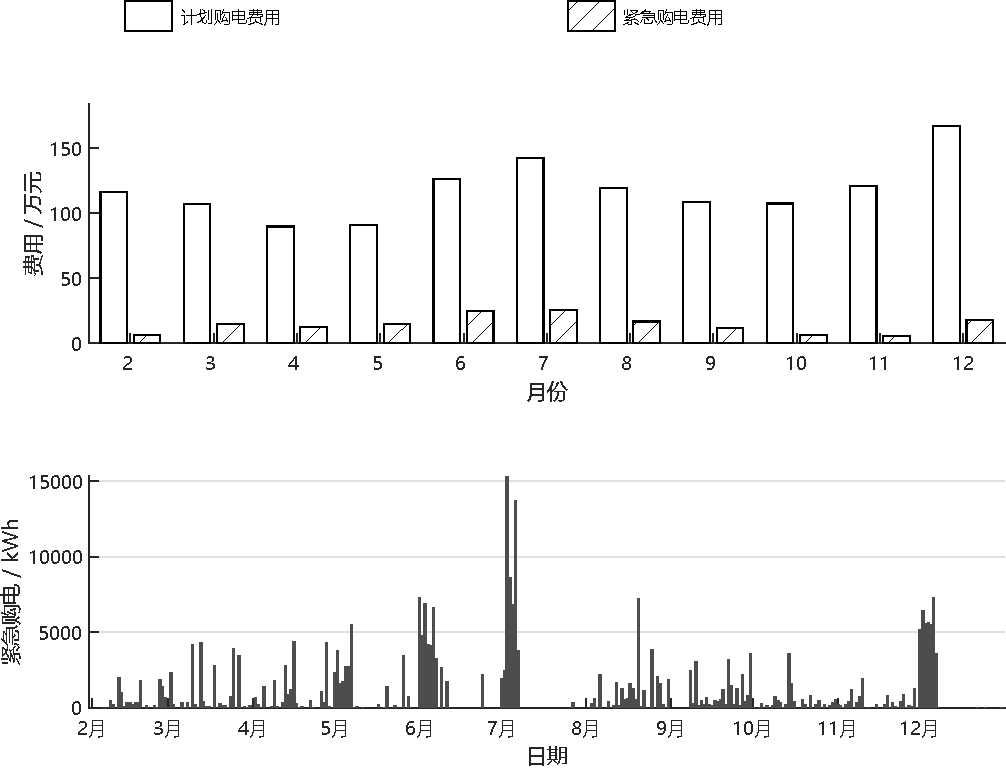
\includegraphics[width=\textwidth,height=.40\textheight,keepaspectratio]{figures/q2_year.pdf}
\caption{问题二的月度费用与每日紧急购电量。}\label{fig:q2year}
\end{figure}
\begin{figure}[htbp]\centering
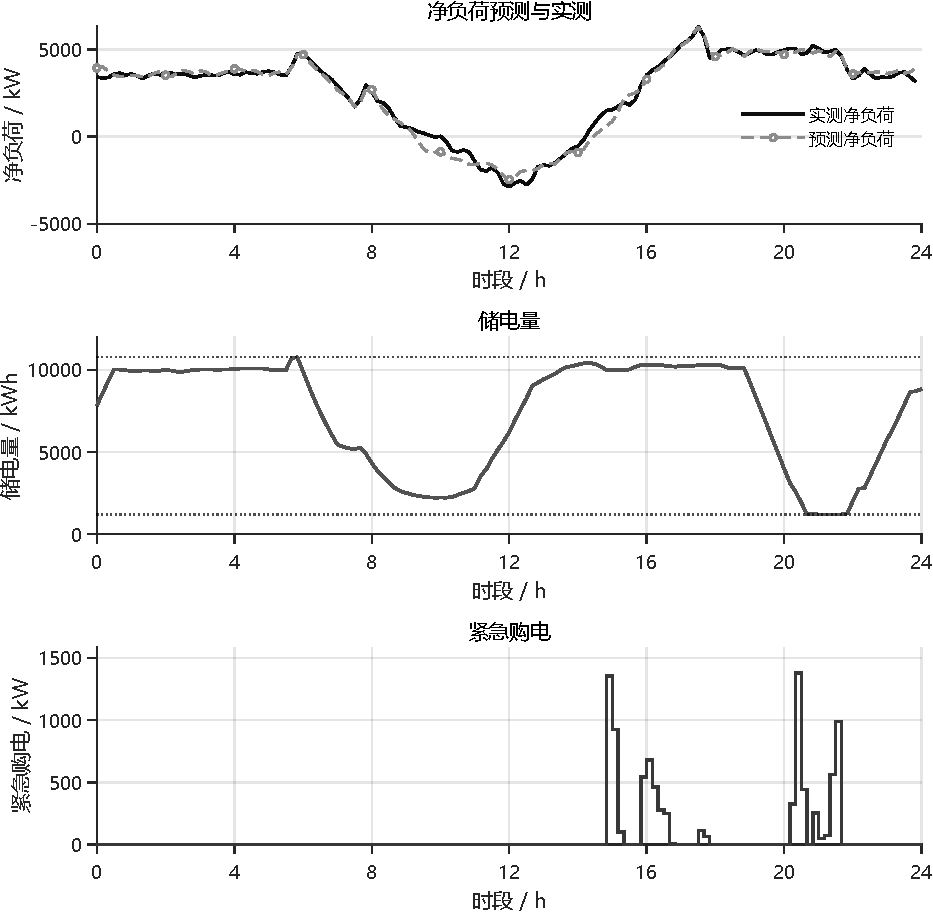
\includegraphics[width=\textwidth,height=.48\textheight,keepaspectratio]{figures/q2_day_20250923.pdf}
\caption{09-23的净负荷预测偏差、实际储电量与紧急购电响应。}\label{fig:q2response}
\end{figure}
